\documentclass[answers]{exam}
\usepackage{../../template}
\title{Problem Set 2}
\author{niceguy}
\begin{document}
\maketitle

\begin{questions}

\question{For the diode attenuator circuit and input waveform shown below, sketch the output voltage waveform, $v_o(t)$. Clearly label all key points on the graph. Assume that the diode has a forward-bias voltage of 0.7V when conducting a current of 1mA, and thermal voltage $V_T= 25\unit{mV}$ at room temperature. Assume also that capacitor C has a very large value. (Hint: it can be shown that the small-signal diode model is valid here.)}

\begin{center}
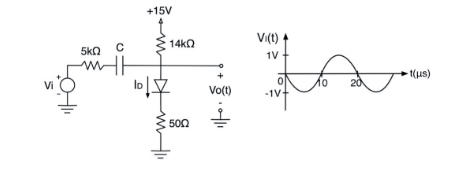
\includegraphics{q1.png}
\end{center}

\begin{solution}
    We start with DC analysis. This is because for the AC analysis, we need to use a small signal approximation. \\
    We can ignore the left hand side, since there is no current through a capacitor when voltage is constant. The voltage drop at the diode is 0.7V. Solving for current,
    $$I_D = \frac{15 - 0.7}{14 + 0.05} \approx 1\unit{mA}$$
    which justifies the assumption of a 0.7V voltage drop. \\
    For AC analysis, the resistance of the linear model is
    $$r_d = \frac{V_T}{I_D} = \frac{25 \times 10^{-3}}{1 \times 10^{-3}} = 25\unit{\Omega}$$
    We assume the capacitor shorts, since we are only concerned with a DC circuit. We turn off the 15V source, and approximate the 14k resistor as an insulator. This becomes a voltage divider, so the amplitude becomes
    $$1 \times \frac{25 + 50}{25 + 50 + 5000} = 15 \times 10^{-3}\unit{V}$$
    By superposition,
    $$V_0 = 0.7 \pm 15 \times 10^{-3}$$
\end{solution}

\question{For each circuit (1-4) shown below, circle the matching voltage transfer characteristic (a-d)}

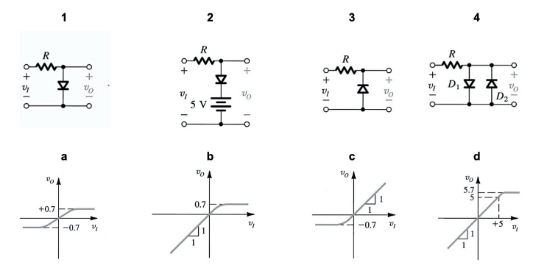
\includegraphics{q2.png}

\begin{solution}
    For 1, consider when the diode is off. Then $v_o = v_i$, and its behaviour at negative $v_i$ would be $y=x$. When the diode is on, $v_o = 0.7\unit{V}$, which happens when $v_i$ is 0.7 or more. Hence the answer is b. \\
    For 2, the diode is off for $v_i \leq 5\unit{V}$. If it is on, adding 5 to the voltage drop 0.7, we have $v_o = 5.7\unit{V}$ when $v_i \geq 5.7\unit{V}$. Hence the answer is d. \\
    For 3, when the diode is off, $v_i = v_o$. This is when $v_i > -0.7\unit{T}$. If it is on, then $v_o = -0.7\unit{V}$. The answer is then c. \\
    For 4, the diodes are off when voltage difference is not yet 0.7 across the diodes. Hence for $|v_i| \leq 0.7\unit{V}$, then $v_o = v_i$. With greater voltages, voltage drop is 0.7V, so $v_o = 0.7\unit{V}$. Similarly, for lower voltages, $v_o = -0.7\unit{V}$. The answer is hence a.
\end{solution}
\end{questions}

\end{document}
